\documentclass[14pt,a4paper,magis]{dipNSU}%загрузка класса. базовый класс -- extreport 
%magis -- для магистратуры bach -- для бакалавриата
\usepackage{amsmath,amssymb,amsfonts}%математика
\usepackage{xcolor}%цвета
\usepackage{lipsum} % for dummy text only
\usepackage[colorlinks = true,
linkcolor = red,
urlcolor  = blue,
citecolor = blue,
anchorcolor = blue]{hyperref}% \href ссылки

\usepackage{setspace}%установка межстрочного интервала
\usepackage{tabularx}%окружение таблиц tabularx
\usepackage{multirow} %объединение строк в таблицах
\usepackage{booktabs}%для всяких украшательств в таблицах (\toprule,\midrule ...)
\usepackage{float} %работа с ``плавающими'' объектами [H]
\usepackage{graphicx}% графика
\usepackage{wrapfig}%картинки с обтеканием

%\usepackage{minted}%листинг кода

%мощный пакет для построения графики разной степени сложности. В обычных текстах обычно не нужен
\usepackage{tikz}
\usepackage{smartdiagram}
\usetikzlibrary{positioning}
\usetikzlibrary{decorations} 
\usetikzlibrary{shapes,arrows}
\usepgflibrary{arrows.meta}
\usetikzlibrary{arrows.meta}
\usetikzlibrary{bending}
\usetikzlibrary{graphs}
\usetikzlibrary{decorations.pathmorphing}
\usetikzlibrary{calc,patterns,angles,quotes}

%вставить список используемых дополнительных пакетов
\graphicspath{{figures/}}% путь к рисункам относительно данного документа

\UpperOrganization{МИНИСТЕРСТВО НАУКИ И ВЫСШЕГО ОБРАЗОВАНИЯ РОССИЙСКОЙ~ФЕДЕРАЦИИ}%минобр
\OrganizationType{ФЕДЕРАЛЬНОЕ ГОСУДАРСТВЕННОЕ АВТОНОМНОЕ ОБРАЗОВАТЕЛЬНОЕ УЧРЕЖДЕНИЕ ВЫСШЕГО ОБРАЗОВАНИЯ}%тип организации
\Organization{<<НОВОСИБИРСКИЙ НАЦИОНАЛЬНЫЙ ИССЛЕДОВАТЕЛЬСКИЙ ГОСУДАРСТВЕННЫЙ УНИВЕРСИТЕТ>> (НОВОСИБИРСКИЙ ГОСУДАРСТВЕННЫЙ УНИВЕРСИТЕТ, НГУ)}%полное название университета
\Faculty{ФИЗИЧЕСКИЙ}%название факультета
\Department{ФИЗИКИ ПЛАЗМЫ}%название кафедры


\title{Шаблон выпускной квалификационной работы}%заголовок курсовой
\author{Анненкова Владимира Вадимовича}%ФИО автора в родительном падеже полностью


\Superviser{ФИО руководителя}%руководитель
\SuperviserDegree{д.ф.-м.н., профессор}%учёная степень руководителя
\SuperviserWorkPlace{г.н.с., ИЯФ СО РАН}

\DepHeadDegree{к.ф.-м.н.}
\DepHeadWorkPlace{в.н.с., ИЯФ СО РАН}
\DepHead{Беклемишев А.Д.}




\KeyWords{Физика плазмы, численное моделирование, \LaTeXe}%ключевые слова


\RefSource{ref}%название файла с библиографией
\SetPDFmeta%установить метаданные pdf файла

%\makeatletter
%\newcommand\thefontsize[1]{{#1 The current font size is: \f@size pt\par}}
%\makeatother


\begin{document}
% \maketitle%Создать титульный лист


%команда \input вставляет заместо себя содержимое указанного файла


{
	\hypersetup{linkcolor=black}%чёрный цвет текста
	\tableofcontents%Сгенерировать оглавление
}


%\Definitions%определения, используемые в работе. Формально в ГОСТе такой пункт есть, реально в дипломной его использовать особого смысла нет
%\Introduction

Это шаблон ВКР, разработанный на основе требований  ГОСТ и деканата \href{http://www.phys.nsu.ru/department/index.php/diplomnikam}{http://www.phys.nsu.ru/department/index.php/diplomnikam}

Также в данном шаблоне содержится некоторое количество примеров  использования \LaTeX'а при вёрстке текста и ссылки на различные полезные источники.

%Введение	
%\chapter{Основная часть}\label{ch:ch1}

Пример главы%глава основной части
%
\chapter{Об этом шаблоне}\label{ch:about}


Данный шаблон создан на основе \href{https://docs.cntd.ru/document/1200026224}{ГОСТ 7.32-2001} ''Отчет о научно-иссле\-до\-ва\-тельской работе. Структура и правила оформления'' и рекомендаций деканата ФФ НГУ:

\href{http://www.phys.nsu.ru/main/index.php/main/news/652-2016-03-01-news-kursovye}{\small http://www.phys.nsu.ru/main/index.php/main/news/652-2016-03-01-news-kursovye}

Настоятельно рекомендуется ознакомиться с этими двумя ресурсами.

Шаблон предназначен для вёрстки посредством \verb*|pdflatex| или \verb*|xelatex| и \verb*|bibtex| (библиография)

Необходимые файлы шаблона:
\begin{enumerate}
	\item \verb*|kurs3.cls| --- настройки класса: объявление вспомогательных команд, настройка оформления и титульного листа;
	\item \verb*|Preamble.tex| --- файл с перечислением подключаемых пакетов;
	\item \verb*|ugost2008.bst| --- стилевой пакет библиографии по ГОСТу 7.0.5-2008. Необходим при вёрстке на локальном ПК --- при использовании \href{https://www.overleaf.com}{overleaf} не нужен. Он там есть по-умолчанию.
	\item \verb*|kurs3temp.tex| --- основной документ, в который подключаются остальные файлы и сам текст;
	\item  \verb*|ref.bib| --- файл с библиографией в формате \verb*|bibtex|'а.
\end{enumerate}

При вёрстке \verb*|pdflatex|'ом шаблон по-умолчанию использует шрифт с засечками Computer Modern Roman (CMR). Это не Times New Roman (TMN) (проприетарный шрифт), который указывается в различных требованиях и ГОСТах. Отдельный вопрос почему он там указывается. Скорее всего фактически имелся ввиду ''шрифт с засечками''. Во времена написания требований офисный документооборот осуществлялся с помощью ПО Microsoft, в котором этот шрифт был основным шрифтом с засечками. На практике проблем с использованием CMR обычно не бывает (особенно в курсовых работах).

Если всенепременно хотите использовать TMN, то есть два пути:

\begin{enumerate}
	\item Если использовать \verb*|pdflatex|, то нужно в файле  \verb*|kurs3.cls| раскомментировать строки
	
	\verb*|\RequirePackage[math]{pscyr}|
	
	\verb*|\renewcommand{\rmdefault}{ftm}|
	
	Это включит использование пакета \verb*|pscyr|, который предварительно нужно установить на Вашу ОС. Этот пакет предоставляет также другие интересные шрифты, например шрифт ''как в старых учебниках'':
	
	 \verb*|\renewcommand{\rmdefault}{fac}|
	\item \verb*|xelatex| позволяет использовать в \verb|.tex| документах системные шрифты. Шаблон настроен таким образом, что при вёрстке им автоматически будет выбрано использование системного шрифта TNR (он должен быть установлен!).
\end{enumerate}

Также этот шаблон успешно верстается в онлайн системе overleaf (кроме режима с использованием pscyr). 

\newpage
Список команд, введёных в данном шаблоне и не являющихся стандартными для \LaTeX:
\begin{enumerate}
	\small
	\setlength\itemsep{-0.3cm}
	\item \verb*|\SetPDFmeta| --- установка метаданных pdf документа
	\item \verb*|\Organization| --- переменная для хранения названия организации
	\item \verb*|\OrganizationType| --- тип организации
	\item \verb*|\UpperOrganization| --- вышестоящая организация
	\item \verb*|\Faculty| --- название факультета
	\item \verb*|\Department| --- название каферды
	\item \verb*|\Superviser| --- фамилия и инициалы руководителя
	\item \verb*|\SuperviserDegree| --- учёная степень и звание (если есть) руководителя
	\item \verb*|\SuperviserWorkPlace| --- должность и место работы руководителя
	\item \verb*|\DepHead|  --- фамилия и инициалы зав. кафа
	\item \verb*|\DepHeadDegree| --- учёная степень и звание (если есть) зав. кафа
	\item \verb*|\DepHeadWorkPlace| --- должность и место работы зав. кафа
	\item \verb*|\RefSource| --- название файла с библиографией
	\item \verb*|\ChapterWithoutNum| --- вспомогательная команда для форматирования заголовка раздела без номера (Введение и т.п.)
	\item \verb*|\References| --- создания списка литературы
	\item \verb*|\Definitions| --- заголовок Определения с добавлением в оглавление без номера
	\item \verb*|\Abbreviations| --- заголовок Сокращения и обозначения с добавлением в оглавление без номера
	\item \verb*|\Introduction| --- заголовок Введение с добавлением в оглавление без номера
	\item \verb*|\Conclusion| --- заголовок Заключение с добавлением в оглавление без номера
	\item \verb*|\Appendix| --- заголовок Приложение с добавлением в оглавление без номера, с увеличением счётчика
\end{enumerate}%об этом шаблоне
%главы с примерами использования LaTeX'а
%заместо этих и других глав ставьте свои

\chapter{Структура геометрического решателя}\label{ch:geomsolver}
% Описание главы

Решатель геометрических ограничений представляет собой программное обеспечение (отдельное приложение или программная библиотека), который позволяет создавать задачу геометрических ограничений и соответственно её решать. Основной интерес представляет внутреннее устройство решателя, которое будет рассмотрено в данной главе. Для удобства представления,  решатель можно структурно разделить на три уровня: верхний, средний и нижний. Эти уровни работают последовательно и различными способами преобразуют исходную задачу, что в итоге приводит к её решению. Решение задачи, в зависимости от исхода может быть получено на разных уровнях. Далее будет рассмотрен каждый из представленных уровней.




\section{Верхний уровень}
Данный уровень представляет собой набор модулей, которые работают с представлением задачи в виде набора геометрических объектов и ограничений связывающих их, которые могут быть представлены в виде  мультиграфа, как на рисунке \ref{fig:im1}. Вершинами такого графа являются геометрические объекты, а рёбра соответствуют геометрическим ограничениям заданным между парой объектов (или в случае ограничений действующих на один объект, ребро замыкается на одной вершине). 

\begin{figure}[h]
	\centering
	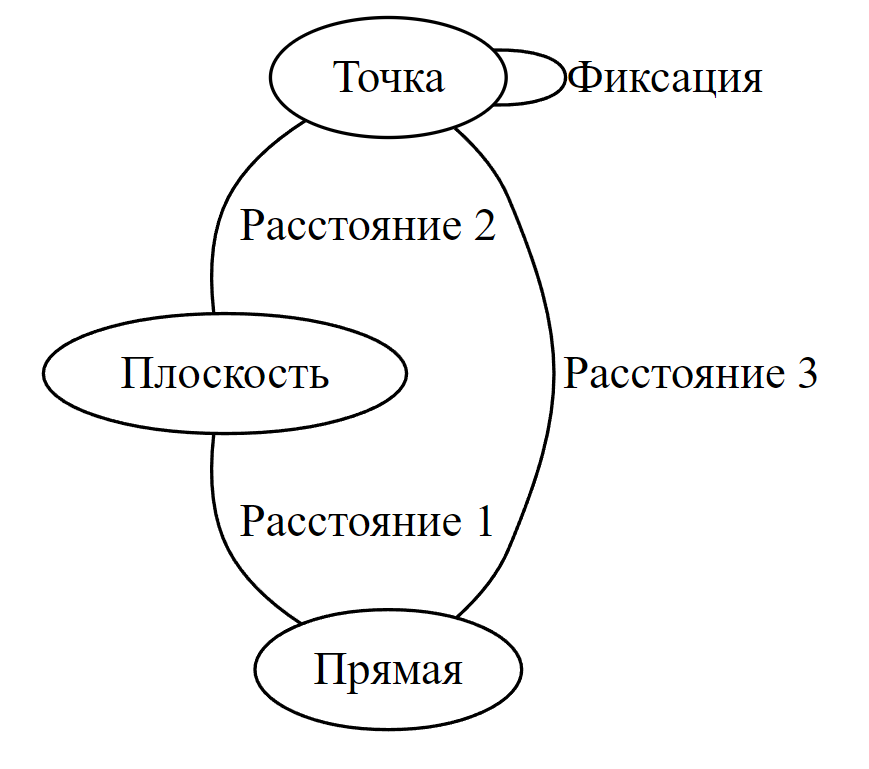
\includegraphics[width=0.5\linewidth]{figures/fig_1_model_graph.png}
	\caption{Пример графа простой геометрической модели}
	\label{fig:im1}%ссылка на картинку
\end{figure}

На данном уровне работает несколько модулей. Важное значение имеет модуль \textit{геометрической декомпозиции}, который способен разделять задачу на подзадачи меньшего размера, что позволяет достичь уменьшения времени решения и увеличения вероятности того, что  решение будет найдено. На этом уровне, также может происходить аналитическое решение небольших задач, исходя из геометрических соображений. Результатом работы этого уровня является одна или несколько подзадач, которые далее требуют непосредственного решения. Также стоит отметить, что на данном этапе возможен исход, при котором исходная задача может и не измениться. Результат работы модуля в виде набора геометрических объектов и ограничений, далее обрабатывается средним уровнем.

Помимо модуля геометрической декомпозиции на данном уровне находится \textit{модуль трансформации}. Его задачей является преобразование сложных ограничений в набор элементарных ограничений. Таким образом, некоторые из поддерживаемых ограничений реализуются в виде набора других более простых ограничений, и отвечает за такое преобразование рассматриваемый модуль. 




\section{Средний уровень}\label{sec:middle_level}
На данном уровне происходит преобразование задачи удовлетворения геометрических решений к алгебраической задаче решения нелинейной системы алгебраических уравнений (далее для краткости СНАУ). Данным преобразованием занимается модуль генерации системы уравнений, который принимает геометрическую модель в виде графа объектов и ограничений, а на выходе предоставляет СНАУ. Помимо данного модуля, к среднему уровню можно отнести так же модули валидации и нормализации. 

\textit{Модуль генерации систем уравнений} является основой среднего уровня. Именно тут происходит основное преобразование задачи удовлетворения геометрических ограничений в задачу решения СНАУ. Данный модуль работает в два этапа. Сначала происходит моделизация геометрических объектов, т.е. описание положения геометрических объектов с помощью набора переменных. Далее для каждого ограничения из задачи генерируется одно или несколько нелинейных, в общем случае, уравнений относительно переменных, с помощью которых описываются геометрические объекты задачи. Подробно устройство данного модуля будет описано в главе \ref{ch:modeler}.

\textit{Модуль нормализации} отвечает за приведение параметров ограничений и объектов к некому каноническому виду, на который опирается модуль генерации уравнений. Параметрами объектов являются их координаты, вектора направлений и для некоторых объектов радиус (или даже радиусы). И например, вектора направлений необходимо нормировать, поскольку все генерируемые уравнения полагаются на единичную длину таких векторов. Не числовыми параметрами ограничений являются такие сущности как выравнивание (т.е. для ограничений в которых направляющие вектора параллельны, этот параметр регулирует направленность этих векторов), ориентация (применима в сосновом для ограничений расстояния и указывает положения объектов относительно нормали одного из них) и др. Также у некоторых ограничений, называемых параметрическими имеются вещественные параметры. К таким ограничениям относят расстояние, угол и радиус. Так же к параметрам ограничений можно отнести такие сущности как вспомогательные точки. Они позволяют конкретизировать точку на поверхности в которой будет удовлетворяться заданное ограничение. Все описанные параметры, в существенном ряде случаев требуют приведения к каноническому виду. Так например, вспомогательные точки обычно перемещаются из заданного пользователем положения в ближайшее положение на поверхности. Или же, например, отрицательное расстояние переводится в положительное и параметр ориентации для расстояние изменяется на противоположенное значение. Данный модуль, отнесён к среднему уровню на основании того, что он не преобразует модуль структурно, т.е. в ходе преобразований не изменяется число и тип объектов, а также не изменяются аргументы ограничений, в отличии от модуля геометрической декомпозиции. Также данный модуль обладает "знанием" о каноническом виде ограничений и объектов, на которое полагается модуль генерации уравнений. 

Ещё одним модулем среднего уровня является \textit{модуль валидации}. Данный модуль отвечает за проверку ограничений из модели на удовлетворенность. Таким образом результатом работы модуля является статус (в простейшем случае двузначного тип) о удовлетворенности всех ограничений. Помимо статуса, модуль выдаёт также численную меру удовлетворенности ограничений. Причём в данную меру входят два параметра: угловая и линейная погрешности. Угловая погрешность вычисляется для векторов направлений, а линейная вычисляется для координат объектов. Тем самым данный модуль, используется в двух случаях. Во-первых для проверки корректности численного решения (т.е. дополнительная проверка помимо невязки самих уравнений), что позволяет легче обнаруживать ошибки в модуле генерации уравнений так и в модуле решения СНАУ. Во-вторых, этот модуль требуется в самом начале работы геометрического решателя, чтобы избежать дальнейшей работы, в случае если пользователь задал изначально удовлетворённую модель. Этот модуль отнесён к среднему уровню, поскольку он в значительной степени согласован с модулем генерации уравнений, т.к. погрешности для ограничений вычисляются подобно вычислению невязки в уравнениях, описывающих данное ограничение.




\section{Нижний уровень} \label{sec:low_level}
Данный уровень ответственен за решение СНАУ, которая генерируется на среднем уровне. Представителями этого уровня являются модули решения системы нелинейных уравнений и алгебраической декомпозиции. 

\textit{Модуль решения СНАУ} реализует итеративный алгоритм Ньютона - Рафсона. Выбор этого метода обусловлен тем, что он способен решать как переопределенные, так и недоопределенные системы нелинейных уравнений \textbf{[тут нужна ссылка на источник подтверждающий мои слова]} и хорошо-определенные системы тоже. Данный алгоритм требует вычисления якобиана системы на на каждой итерации. В некоторых модификациях якобиан обновляется лишь через несколько итераций. Помимо этого, на каждой итерации решается СЛАУ, матрицей которой как раз и является якобиан системы. Эта операция является самой дорогой в терминах вычислительной сложности, поэтому сложность решения СНАУ оценивается как \cite{GoluVanl96}:
\begin{equation*}
    O(L \cdot m \cdot n^2)
\end{equation*}
если $m > n$, иначе:
\begin{equation*}
    O(L \cdot n \cdot m^2)
\end{equation*}
где $n$ -- число переменных, $m$ -- число уравнений, $L$ -- число итераций метода Ньютона. Число итераций метода в общем случае неизвестно, т.к. он не гарантирует сходимости с произвольной начальной точки. Поэтому оно ограничивается сверху эмпирически подбираемым значением, которое в худшем случае не будет приводить к существенным задержкам, когда метод не сходится. Помимо ограничения сверху, могут быть использованы различные эвристики, для преждевременной остановки решения. Например, если несколько итераций подряд норма шага метода близка к нулю, то можно прекратить решение. \textbf{/* Здесь также можно написать про ещё одну эвристику с рекордом на N прошлых итерациях*/}

\textit{Модуль алгебраической декомпозиции} производит разбиение, другими словами декомпозицию, системы уравнений на несколько подсистем, которые далее решаются по отдельности, в заданном порядке. В основе работы модуля лежит алгоритм декомпозиции двудольных графов Далмейджа-Мендельсона \cite{dulmage1958coverings}. Алгоритмическая сложность такой декомпозиции меньше чем сложность алгоритма решения СНАУ. таким образом этот модуль позволяет в ряде случаев достичь ускорения при решении, по сравнению с решением системы уравнений целиком. Для своей работы, данный алгоритм требует поиска переменных, от которых зависит каждое их уравнений системы. Это требуется для построения двудольного графа зависимостей для системы уравнений. Далее, алгоритм предоставляет набор подсистем, которые необходимо решить в заданном алгоритмом порядке. Более детально рассматриваемый модуль будет описан в одной из следующих секций.

\chapter{Модуль генерации уравнений для геометрических ограничений}\label{ch:modeler}

Как было описано в главе \ref{ch:geomsolver}, задача удовлетворения геометрических ограничений в итоге сводится к численному решению СНАУ. Но для того, чтобы получить СНАУ необходимо, во-первых, представить элементарные геометрические объекты и тела в виде набора переменных. Телом в данном случае называется сложный геометрический объект, представляющий собой набор элементарных геометрических объектов неподвижных относительно друг друга. Во-вторых, для каждого из ограничений генерируется набор уравнений относительно переменных, соответствующих аргументам ограничения. Таким образом в итоге получается система уравнений, описывающая задачу удовлетворения геометрических ограничений. Далее будет представлен набор поддерживаемых геометрических объектов и ограничений, а также описаны способы представление гомерических объектов и в конце будут описаны подходы и особенности описания ограничений набором алгебраических уравнений.

\section{Обзор поддерживаемых объектов и ограничений}

В рамках данной в модуле генерации уравнений была реализована поддержка геометрических объектов и ограничений, представлены в таблице \ref{tab:supp_obj_and_constr}. Ограничения могут задаваться между представленными объектами, если это имеет смысл. Например, между двумя точками ограничение угла не определено. В дальнейшем, планируется поддержка дополнительных геометрических объектов, например сфера, цилиндр и др. Но Описанные далее способы моделизации объектов и методы генераций уравнений могут быть также применены и к таким объектам.

\begin{table}[htbp]
	\caption{Поддерживаемые геометрические объекты и ограничения}
	\label{tab:supp_obj_and_constr}
	\begin{tabularx}{\textwidth}{XX}
		\toprule
		\textbf{Объекты} & \textbf{Ограничения}\\
		\hline
		точка       & совпадение\\
		прямая      & расстояние\\
		плоскость   & касание   \\
		окружность  & фиксация  \\
		            & угол      \\
		            & параллельность\\
		            & перпендикулярность\\
		% & \\
		\bottomrule
	\end{tabularx}
\end{table}

В разделе \ref{sec:middle_level} были упомянуты параметры геометрических ограничений. В целом для ограничений существуют следующие параметры: \textit{выравнивание}, \textit{ориентация} и \textit{вспомогательная точка}. Параметры выравнивание и ориентация могут принимать три значение: положительное, отрицательное и неопределённое. Параметр выравнивание отвечает за поведение направляющих векторов, когда ограничение требует параллельности направляющих векторов обоих геометрий. Например расстояние между плоскостями требует параллельности их нормалей, и в таком случае положительное выравнивание означает со-направленность нормалей, а отрицательное наоборот. В случае неопределенного выравнивания допустимы оба варианта. Параметр ориентация определён только для ограничения расстояния, хотя бы одним аргументом которого является поверхность, и отвечает он за положение объекта относительно нормали поверхности. Например, для ограничения расстояния между плоскостью и точкой возможны два решения: точка находится спереди плоскости (т.е. нормаль направлена к точке) или же точка находится за плоскостью. В общем случае, положительная ориентация означает, что нормаль указывает на объект, а   с отрицательным значение -- наоборот. В таблице \ref{tab:constr_params} указано, какие параметры могут быть у каждого из ограничений. Также, часть ограничений не имеет параметров. А ограничение фиксации имеет собственный уникальный параметр, который позволяет задать полную, или частичную фиксацию объекта.   

\begin{table}[htbp]
    \renewcommand{\arraystretch}{1.4}
	\caption{не числовые параметры ограничений: В -- выравнивание, О -- ориентация, ВТ -- вспомогательная точка, ТФ -- тип фиксации}
	\label{tab:constr_params}
	\begin{tabularx}{\textwidth}{XX}
		\toprule
		\textbf{Ограничение} & \textbf{Параметры}\\
		\hline
		совпадение         & В, ВТ      \\ \hline
	    расстояние         & В, ВТ   \\ \hline
	    касание            & В, О, ВТ   \\ \hline
	    фиксация           & ТФ         \\ \hline
	    угол               & --         \\ \hline
	    параллельность     & В          \\ \hline
	    перпендикулярность & --         \\
	    \bottomrule
	\end{tabularx}
\end{table}


\section{Способы моделирования геометрических объектов и тел}
Как было упомянуто ранее, в первую очередь для генерации уравнений необходимо задать набор переменных, над которыми и будут далее заданы уравнения. Существует как минимум два подхода к представлению геометрических объектов \cite{ershov2007algorithms}. 

Первый подход основан на представлении искомых координаты элементарных геометрических объектов в виде переменных системы. Например, точку можно представить в виде набора трёх переменных, соответствующих её координатам. Отдельно стоит рассмотреть представление направляющих векторов, т.к. при генерации уравнений очень удобно опираться на единичную длину направляющих векторов. Для гарантии единичной нормы векторов, можно представлять такие вектора в виде двух углов ($\vartheta$ и $\varphi$), как представляется любой вектор в сферической системе координат с единичным радиусом. 

\begin{equation*}
    \begin{matrix}
        & x  = \cos{\varphi} \cdot \sin{\vartheta} \\ 
        & y  = \sin\varphi \cdot \sin\vartheta \\
        & z  = \cos\vartheta
    \end{matrix}
\end{equation*}

Но в таком случае координаты такого вектора выражаются через произведения тригонометрических функции от переменных-улов. И как показывает практика, такой подход обеспечивает более плохую сходимость решателя по сравнению со следующим подходом. В этом случае компоненты вектора являются переменными ($x, y, z$), а для обеспечения единичной нормы такого вектора в систему уравнений добавляется уравнение обеспечивающее единичную норму:  

\begin{equation*}
    x^2 + y^2 + z^2 - 1 = 0
\end{equation*}

Исходя из описанных выше соображений, для каждого из поддерживаемых объектов был выбран следующий способ моделирования -- представления в виде набора переменных:

\begin{itemize}
    \item
        \textbf{Точка} -- координаты самой точки; в итоге \textbf{3} переменных.
    \item
        \textbf{Прямая} -- координаты точки на прямой, направляющий вектор; в итоге \textbf{6} переменных.
    \item
        \textbf{Плоскость} -- расстояние от плоскости до начала координат, нормаль (направляющий вектор); в итоге \textbf{4} переменных.
    \item
        \textbf{Окружность} -- координаты центра, нормаль к плоскости (направляющий вектор), радиус; в итоге \textbf{7} переменных.
\end{itemize}

Вторым походом к моделированию объектов является представление положений объектов в виде трансформаций, описывающих переход положения объекта из исходного в искомое. Трансформация в таком случае представляется в виде поворота и смещения, и её параметры являются переменными, соответствующими геометрическому объекту. Описать трансформацию можно несколькими способами. Первый, и не очень эффективный метод, 12-параметрическое моделирование, когда трансформация представляется виде 9 переменных для матрицы поворота и 3 переменных вектора для смещения:

\begin{equation*}
    R = \begin{pmatrix}
        x_1 & x_2 & x_3\\
        x_4 & x_5 & x_6\\
        x_7 & x_8 & x_9
    \end{pmatrix},
    t = \begin{pmatrix}
        x_{10}\\
        x_{11}\\
        x_{12}
    \end{pmatrix}
\end{equation*}
где, $R$ -- матрица поворота, $t$ -- вектор смещения. Поскольку матрица $R$ должна быть матрицей поворота в трёхмерном пространстве, необходимо чтобы она была ортогональной и её определитель равнялся 1. Для этого необходимо 6 дополнительных уравнений для обеспечения требуемых свойств матрицы $R$.

Другой способ является 6-параметрическим и в нём переменными являются 3 угла Эйлера ($\alpha, \beta, \gamma$), описывающих поворот, а также 3 компоненты вектора смещения ($x, y, z$). Такой подход позволяет избавиться от дополнительных уравнений и и обеспечить меньше количество переменных в системе. Существует 12 возможных описаний матрицы поворота с помощью углов Эйлера \textbf{[ссылка на книгу из статьи на Вики]}, и как показала практика выбор представления матрицы поворота влияет на сходимость численного решения, но это влияние не существенно. Но главной особенностью такого подхода является описание геометрических тел. В таком случае описанная трансформация является общей, для набора геометрических объектов, каждое из которых имеет собственные координаты в локальной системе координат тела. В таком случае координаты любого объекта получаются путём применения трансформации всего тела к локальным координатам объекта. Для описания одного объекта такой подход оказываются не эффективен на практике, т.к. заметно ухудшается сходимость решателя при таком способе моделирования объектов. Поэтому при реализации рассматриваемого модуля был выбран смешанный подход, в котором для моделирования одиночных геометрических объектов используется первый из описанных подходов, а для моделирования геометрических тел используется второй подход. 

\section{Особенности генерируемых уравнений}

Как было описано в разделе \ref{sec:low_level}, для решения СНАУ в разрабатываемом решателе используется метод Ньютона-Рафсона, требующий вычислений якобиана системы уравнений на каждой итерации. Этот факт, приводит к тому, что все генерируемые уравнения должны быть дифференцируемы (т.е. частные производные определены во всей области допустимых значений переменных) по всем переменным, от которых они зависят. В противном случае, появление NaN (Not A Number -- не число) или бесконечных значений в якобиане приводит к некорректному решению СЛАУ и в следствии к расходимости метода Ньютона-Рафсона. Исходя из этого факта, требование дифференцируемости  уравнений на всей области определения существенно и должно учитываться при реализации вычислений. 

Одним из первых мест, где проблемы с дифференцируемостью уравнений возникают проблемы, являются уравнения описывающие расстояние между объектами. Например, расстояние $d_0$ между двумя точками, очевидным образом можно задать уравнением:
\begin{equation}\label{eq:pt_pt_dist_bad}
   \left \|  \Vec{p_1} - \Vec{p_2} \right \|_2 - d_0 = 0
\end{equation}
где: $\Vec{p_1}$, $\Vec{p_2}$ -- координаты первой и второй точки соответственно, $d_0$ -- заданное ограничением расстояние между точками. Но в случае если обе точки совпадают, то все частные производные по компонентам $\Vec{p_1}, \Vec{p_2}$ будут не определены. Такое может происходить в различных случаях. Во-первых, пользователь может задать исходное положение с совпадающими точками (особенно если при построении задачи объекты копируются). Во-вторых, расстояние между точками $d_0$ может быть нулевым. А также, в процессе решения координаты точек могут совпасть. И во всех этих случаях в якобиане системы уравнений появляются NaN значения и метод после этого начинает расходится. Избежать этого, можно с помощью кусочно заданных функций. Так, уравнение \ref{eq:pt_pt_dist_bad} может быть заменено следующим уравнением:

\begin{equation*}\label{eq:pt_pt_dist_good}
\left\{\begin{matrix}
 \left \|  \Vec{p_1} - \Vec{p_2} \right \|_2 - d_0 = 0, 
 & \text{ если }  \left \|  \Vec{p_1} - \Vec{p_2} \right \|_2 \leq \veps \\ 
 
 \left \|  \Vec{p_1} - \Vec{p_2} \right \|_2^2 - d_0^2 = 0, 
 & \text{ иначе }
  
\end{matrix}\right.    
\end{equation*}
где: $\veps$ -- допустимая погрешность решения. Можно заменить это кусочно заданное уравнение на второе, не потеряв свойство дифференцируемости, однако, на практике с кусочно заданной функцией решатель сходится в лучше. Подобный подход, также используется при описание других ограничений расстояния, а именно там, где в уравнении вычисляется евклидова норма вектора. Например, это используется в расстоянии между прямыми, между точкой и прямой, между точкой и окружностью и т.д. 

\textcolor{red}{\textbf{TODO: стоит подумать, нет ли ещё мест, где возникали проблемы с дифференцированием}}

\section{Выбор описания ограничений}
Ограничения описываются набором уравнений не единственным образом. Как минимум, потому, что если имеется несколько уравнений, описывающих данное ограничение, то все уравнения можно объединить в одно путём суммирования квадратов левых частей уравнений. Но уменьшение числа уравнений не обязательно приводит к лучшей сходимости решателя. Поэтому вариативность в способах описания ограничений даёт пространство для оптимизаций генерируемых уравнений, на уже существующей тестовой базе. Далее будут рассмотрены случаи, в которых было найдено более успешное описание ограничений, которое увеличило процент успешно решённых тестов на индустриальной тестовой базе. 

\textbf{Совпадение двух точек.} Данное ограничение можно трактовать как нулевое расстояние между точками и воспользоваться уравнениями \ref{eq:pt_pt_dist_good}. Но существует описание, при использовании которого процент успешно решенных тестов выше:
\begin{equation*}
    \left\{\begin{matrix}
    a_x - b_x & = 0\\
    a_y - b_y & = 0\\
    a_z - b_z & = 0
    \end{matrix}\right.
\end{equation*}
где: $\vec{a}, \vec{b}$ -- координаты двух точек. Этот пример, наглядно показывает, что минимизация числа уравнений в системе не лучший подход к выбору описания ограничений.

%Можно предположить, почему такое описание более удачно, воспользовавшись терминами степеней свободы объектов. Так, у двух свободных точек 6 степеней свободы. Однако ограничение совпадения снимает 3 степени свободы, т.к. положение одной из точек полностью определено положением другой. Соответственно // Крайне спекулятивный момент, который я е смогу ничем подтвердить, а значит писать это вряд-ли стоит

\textbf{Совпадение прямых.} Подобно совпадению двух точек, совпадение прямых можно описать б\'oльшим числом уравнений, чем расстояние между прямыми. Для этого введём обозначения: $\vec{d}$ -- направляющий вектор одной из прямых, $\vec{\Delta}$ -- вектор разности точек, лежащих на соответствующих прямых, $\vec{c} = \vec{\Delta}\times \vec{d} $. Тогда набор уравнений, удовлетворяющий ограничение совпадения, имеет вид:
\begin{equation*}
        c_x, c_y , c_z = 0
\end{equation*}
Помимо этого необходим набор уравнений обеспечивающий коллинеарность направляющих векторов прямых.

\textbf{Параллельность направляющих векторов.} Многие ограничения (совпадение, расстояние, касание и параллельность) требуют коллинеарности направляющих векторов. И на практике, в большинстве случаев оказывается более эффективным набор уравнений, по сравнению с одним уравнением, использующим скалярное произведение векторов. Также нужно учитывать параметр выравнивания, заданный в ограничении. Так при \textit{положительном} или \textit{отрицательном} выравнивании эффективным оказывается набор следующих уравнений:
\begin{equation*}
    \left\{\begin{matrix}
    a_x \pm b_x & = 0\\
    a_y \pm b_y & = 0\\
    a_z \pm b_z & = 0
    \end{matrix}\right.
\end{equation*}
где: $\vec{a}, \vec{b}$ -- направляющие вектора, знаку "$+$" соответствует случай отрицательного, а знаку "$-$" положительного выравнивания. В случае \textit{неопределённого} выравнивания эффективным оказывается приравнивание к нулю компоненты векторного произведения $\vec{c} = \vec{a} \times \vec{b}$:
\begin{equation*}
    c_x, c_y, c_z = 0
\end{equation*}

\textbf{Расстояние между параллельными прямыми.}

\textcolor{red}{\textbf{TODO: дописать секцию!}}

\textbf{Возможно стоит ещё описать работу со вспомогательными точками}
\chapter{Модуль алгебраической декомпозиции}\label{ch:algdec}

Данная глава посвящена описанию работы модуля алгебраической декомпозиции, особенностей реализации.

\section{Описание алгоритма}
Работа алгоритма начинается с того, что для каждого из уравнений генерируемой на среднем уровне СНАУ вычисляется набор переменных от которого это уравнение зависит. Вывод переменных зависимости реализуется вручную, путём анализа каждого уравнения. В итоге, получив для каждого уравнения набор переменных, от которых оно зависит, можно построить двудольный граф, который и будет непосредственно участвовать в декомпозиции. Вершинами такого графа являются уравнения и переменные, которые и образуют две доли, а ребро между вершиной-уравнением $y$ и вершиной-переменной $x$ существует тогда, когда уравнение $y$ зависит от переменной $x$. Пример такого графа изображен на рисунке \ref{fig:graph_example}. В дальнейшем, над таким графом выполняется ряд преобразований, который разбивает граф на несколько подграфов, которые соответствуют подсистемам уравнений, которые можно решать по отдельности. 

\begin{figure}[h]
	\centering
	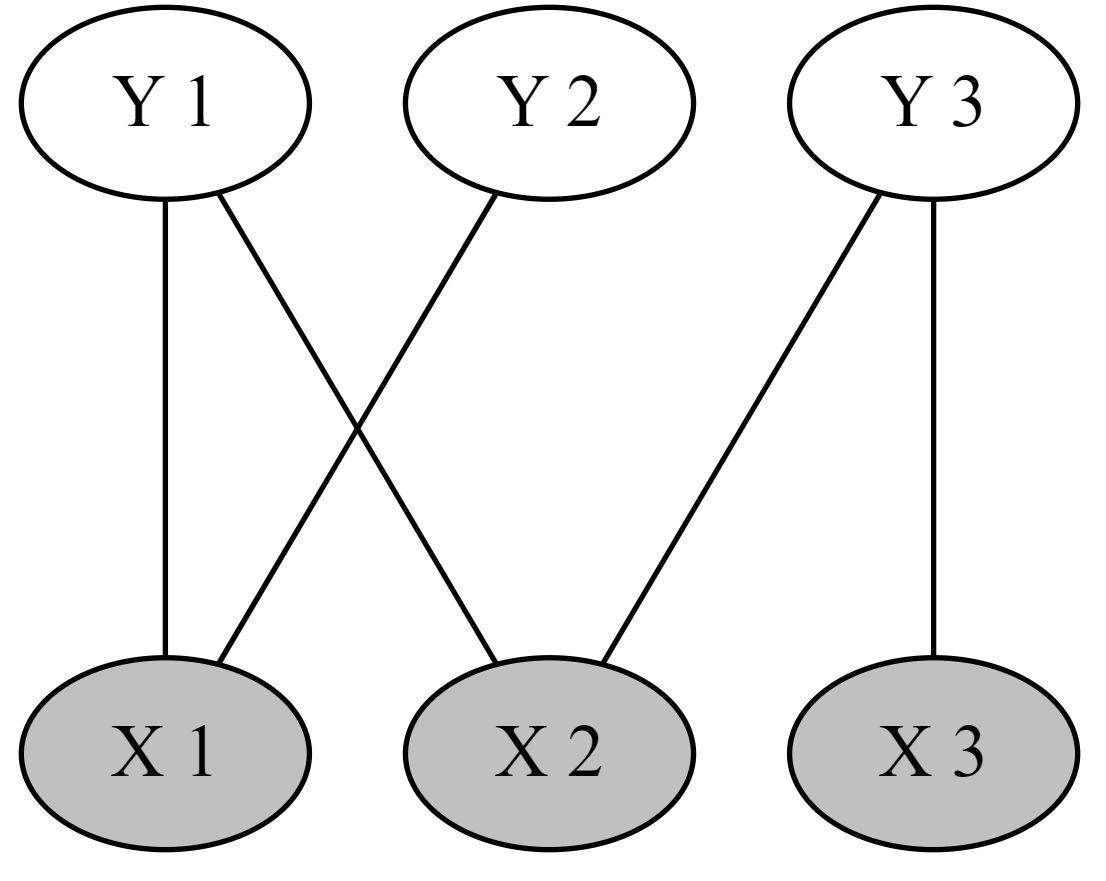
\includegraphics[width=0.3\linewidth]{fig_graph_example.png}
	\caption{Пример графа зависимости уравнений от переменных в системе}
	\label{fig:graph_example}
\end{figure}

Работа алгоритма разделена на две основных части. Сначала производится разделение графа на три подграфа (как минимум один из которых не является пустым) соответствующих пере-, недо- и хорошо-определенным подсистемам. \textit{Хорошо определенной системой} называется такая система уравнений, в графе которого существует идеальное паросочетание. Система уравнений называется \textit{переопределённой}, если число уравнений в ней больше чем число переменных, и наоборот если число переменных меньше числа уравнений, то система называется \textit{недоопределённой} \cite{ait2014reduction}. После первого этапа, если граф хорошо-определённой подсистемы не пуст, то он разбивается на множество хорошо-определённых несократимых подсистем. Несократимость подсистемы означает невозможность разделить подсистему тем же алгоритмом, или же математически это свойство записывается как условие, что для любого подмножества вершин уравнений $Y'$ из уравнений $Y$ выполняется:
\begin{equation*}
 \left|\Gamma(Y') \right| > \left|Y'\right|
\end{equation*}
где: $\Gamma(Y)$ -- множество соседей вершин $Y$, $ \left|Y\right|$ -- мощность множества $Y$.

Второй этап декомпозиции хорошо-определенной подсистемы существенно опирается на предположение о том, что любая хорошо-определённая система имеет хотя бы одно решения. Но в общем случае это не верно, но на практике эффект этого явления слабее чем достигаемое ускорение. В случае не успешного решения одной из подсистем, можно попытаться решить исходную систему уравнений целиком. В таком случае, алгебраическая декомпозиция не уменьшит процент успешно решённых тестов, но ускорение обеспечиваемое декомпозицией также станет меньше, в зависимости от числа тестов, в которых одна из подсистемы была решена не успешно. 

\section{Устройство алгоритма}

Для полного описания обоих частей алгоритма, необходимо ввести следующее преобразование графа $K$:

\textbf{Определение.} Пусть дан граф неориентированный двудольный $G$ и его максимальное паросочетание $M$. Тогда преобразование $K$ переводит граф $G$ в ориентированный двудольный граф $G'$, путём замены всех рёбер из паросочетания $M$ на две дуги $xy$ и $yx$, и ориентированием всех не попавших в паросочетание рёбер от $Y$ к $X$, где $X$ -- вершины-переменные, $Y$ -- вершины-уравнения.

Используя это определение, устройство первой части алгоритма можно записать следующим образом, обозначая исходный граф системы как $G$, граф хорошо-определённой подсистемы как $G_1$,  переопределённой  -- $G_2$, недоопределённой -- $G_3$ \cite{ait2014reduction}:
\begin{enumerate}
    \item 
        Найти максимальное паросочетание $M$ в $G$.
    \item
        Получить ориентированный граф $G'$, применив преобразование $K$ к графу $G$.
    \item
        $G_2$ -- это множество всех потомков от всех истоков в графе $G'$.
    \item
        $G_3$ -- это множество всех предков от всех стоков в графе $G'$.
    \item
        В итоге $G_1 = G - G_2 - G_3$ 
\end{enumerate}
Шаги алгоритма 2--5 могут быть выполнены за время $O(|X| + |Y|)$. А весть алгоритм может быть выполнен за время оцениваемое как $O(|Y|\cdot |X|^\frac{1}{2})$ с использованием алгоритма Хопкрофта — Карпа на шаге 1 \cite{hopcroft1973n}. Важно отметить, что подсистемы $G_2$ и $G_3$ могут содержать в себе несколько независимых компонент. Поэтому имеет смысл также анализировать эти подсистемы, и разбивать их на независимые части. Полученные подсистемы должны решаться в следующем порядке: $G_2, G_1, G_3$.

Вторая часть алгоритма, разбивает подсистему $G_1$ на набор несократимых подсистем, и устроена она следующим образом:
\begin{enumerate}
    \item 
        Найти максимальное паросочетание $M_1$ в $G_1$ (для этого можно использовать уже найденное ранее паросочетание M).
    \item
        Построить ориентированный граф $G_1'$ применяя преобразование $K$ к графу $G_1$.
    \item
        Найти в $G_1'$ компоненты сильной связности $S$, которые и являются несократимыми подсистемами.
    \item
        Для определения порядка решения подсистем из $S$ необходимо произвести топологическую сортировку компонент $S$. Порядок заданный сортировкой, определяет порядок решения систем.
\end{enumerate}
Шаги 2 -- 4 могут быть вычислены за $O(|X| + |Y|)$, с использованием алгоритма Тарьяна \cite{tarjan1972depth} для шагов 3 -- 4, поскольку этот алгоритм гарантирует, что все компоненты в $S$ будут отсортированы.

\textcolor{red}{\textbf{TODO: описать особенности работы с уравнением BoundedValue}}
\chapter{Результаты}\label{ch:results}

Подробные результаты работы модуля алгебраической декомпозиции представлены на рисунке \ref{fig:time_res}, где сравнивается работа модуля без повторной попытки решения с работой решателя без модуля алгебраической декомпозиции. Суммарное ускорение времени решения при включении алгебраической декомпозиции составило:
\begin{itemize}
    \item 
        с повторной попыткой решения: 77\% 
    \item
        без повторной попытки: 81\% 
\end{itemize}

\begin{figure}[h]
	\centering
	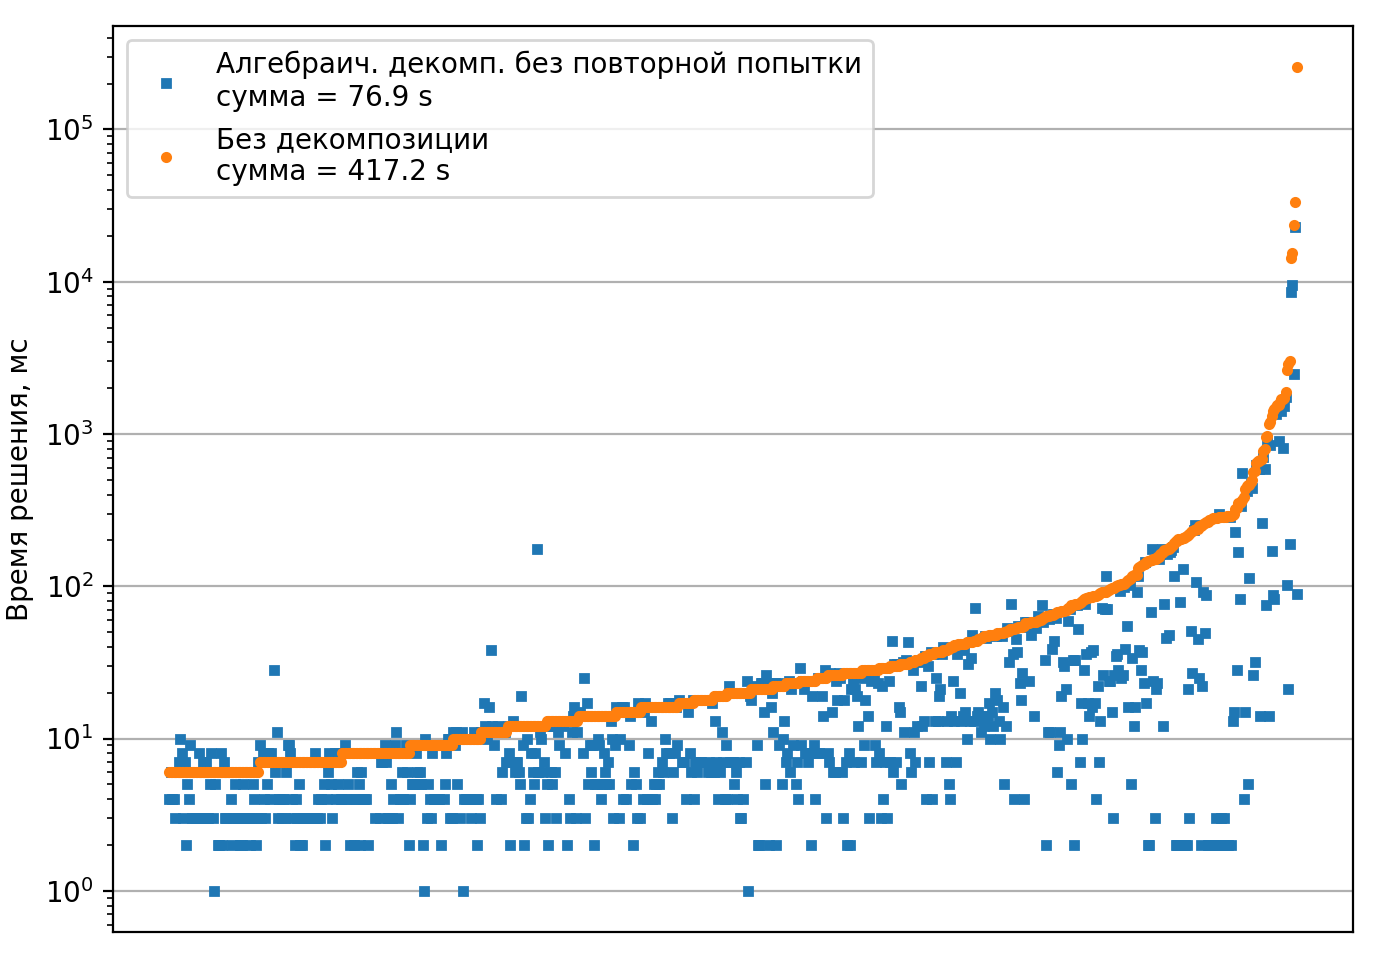
\includegraphics[width=0.6\linewidth]{figures/fig_time_results.png}
	\caption{Результаты работы модуля алгебраической декомпозиции в 3D на индустриальной тестовой базе из ~3000 тестов}
	\label{fig:time_res}
\end{figure}

Процент решенных тестов составил:
\begin{itemize}
    \item с повторной попыткой решения:  95.6\% $\rightarrow$ 97.6\%
    \item  без повторной попытки:  95.6\% $\rightarrow$ 96.7\%
\end{itemize}


%\chapter{Таблицы}\label{ch:tab}
\begin{itemize}
	\item 	\href{http://mydebianblog.blogspot.com/2009/01/tables-in-latex.html}{http://mydebianblog.blogspot.com/2009/01/tables-in-latex.html}
	
	\item 	\href{http://mydebianblog.blogspot.com/2013/01/advanced-tables-in-latex.html}{http://mydebianblog.blogspot.com/2013/01/advanced-tables-in-latex.html} 
\end{itemize}

Для некоторых приведённых примеров требуются пакеты:

окружение таблиц tabularx:\verb|\usepackage{tabularx}|

объединение строк в таблицах:
\verb|\usepackage{multirow}|

для всяких украшательств в таблицах:
\verb|\usepackage{booktabs}|

работа с ``плавающими'' объектами:
\verb|\usepackage{float}|


По ГОСТу оформлены таблицы \ref{tab:GOST1} и \ref{tab:GOST2}.


\begin{table}[ht]
	%\renewcommand{\arraystretch}{1.8} %% increase table row spacing
	%\renewcommand{\tabcolsep}{1cm}   %% increase table column spacing
	\caption{Простая таблица}
	\begin{tabular}{|c|c|r|l|}
		\hline
		раз & два & три & четыре \\
		\hline
		1 & 2 & 3 & 4 \\
		\hline
		пять & шесть & семь & восемь \\
		\hline
		9 & 10 & 11 & 12 \\
		\hline
	\end{tabular}
\end{table}


\begin{table}[H]
		\caption{Такая таблица по ГОСТу}
		\label{tab:GOST1}
	\begin{center}
		\begin{tabular}{|c|c|c|}
			\hline
			\multirow{3}{*}{Размеры нестандартных болтов} & \multicolumn{2}{c|}{Диаметр} \\
			\cline{2-3}
			& Норма & Разброс \\
			\cline{2-3}
			& 10 мм & 1 мм \\
			\hline
		\end{tabular}
	\end{center}
\end{table}

\begin{table}[H]
		\caption{Такая таблица по ГОСТу}
		\label{tab:GOST2}
	\begin{center}
		\begin{tabular}{|c|c|c|}
			\hline
			& \multicolumn{2}{c|}{Диаметр} \\
			\cline{2-3}
			\raisebox{1.5ex}[0cm][0cm]{Нестандартные болты}
			& Норма & Разброс \\
			\hline
			Размеры & 10 мм & 1 мм \\
			\hline
		\end{tabular}
	\end{center}
\end{table}

\begin{table}[htbp]
	\caption{Таблица по ширине страницы}
	\begin{tabularx}{\textwidth}{XXXXX}
		\toprule
		auto & break & case & char & const\\
		%	\hline
		continue   & default   & do & double & else\\
		%	\hline
		\bottomrule
	\end{tabularx}
\end{table}

\begin{table}[htbp]
	\centering
	\caption{Изменённое соотношение ширин столбцов}
	\begin{tabularx}{.85\textwidth}{>{\hsize=0.075\textwidth}XX>{\hsize=0.075\textwidth}XX}
		\toprule
		== & Равно & != & Не равно\\
		> & Больше & < & Меньше\\
		\bottomrule
	\end{tabularx}
\end{table}


\begin{table}[!hbt]
		\caption{Таблица с фиксированной шириной колонок и увеличенным размером строк.}
	\begin{center}
		\renewcommand{\arraystretch}{1.2} %% increase table row spacing	
		\begin{tabular}{|>{\raggedright\arraybackslash}m{3.2cm}|>{\arraybackslash}p{1.9cm}|>{\raggedright\arraybackslash}m{5cm}|>{\raggedright\arraybackslash}m{5cm}|}
			\hline
			\textbf{Величина} & \textbf{Обоз-е} & \textbf{Значение в СИ} & \textbf{Значение в СГС} \\
			\hline
			\textbf{Масса электрона} & $m_e$ &$9.1094\cdot10^{-31}$, кг  & $9.1094\cdot10^{-28}$, г  \\
			\hline
			
		\end{tabular}
	\end{center}
\end{table}	


%\Conclusion

В заключении (выводе) следует четко сформулировать основные выводы, к которым пришел автор. Выводы должны быть краткими и органически вытекать из содержания работы. Разрешается повторить основные выводы соответствующих глав, но при этом предпочтительнее стремиться сделать некоторые обобщения по результатам проведенного исследования в целом.
%Заключение


\References%вставка библиографии. Если библиография не появляется после вёрстки -- вручную запустите bibtex dipTemp.tex

%Приложения (если вдруг нужны)
%\Appendix


Этот элемент структуры работы не является обязательным. Приложения целесообразно вводить, когда автор использует относительно большое количество громоздких таблиц, статистического материала. Такой материал, помещенный в основную часть, затруднил бы чтение работы. Обычно в тексте достаточно лишь сослаться на подобную информацию, включенную в приложение.



\begin{table}[H]
	\caption{Такая таблица по ГОСТу}
	\label{tab:GOST3}
	\begin{center}
		\begin{tabular}{|c|c|c|}
			\hline
			\multirow{3}{*}{Размеры нестандартных болтов} & \multicolumn{2}{c|}{Диаметр} \\
			\cline{2-3}
			& Норма & Разброс \\
			\cline{2-3}
			& 10 мм & 1 мм \\
			\hline
		\end{tabular}
	\end{center}
\end{table}
Ссылка на таблицу в Приложении: Таблица~\ref{tab:GOST3}

\begin{figure}[h]
	\centering
	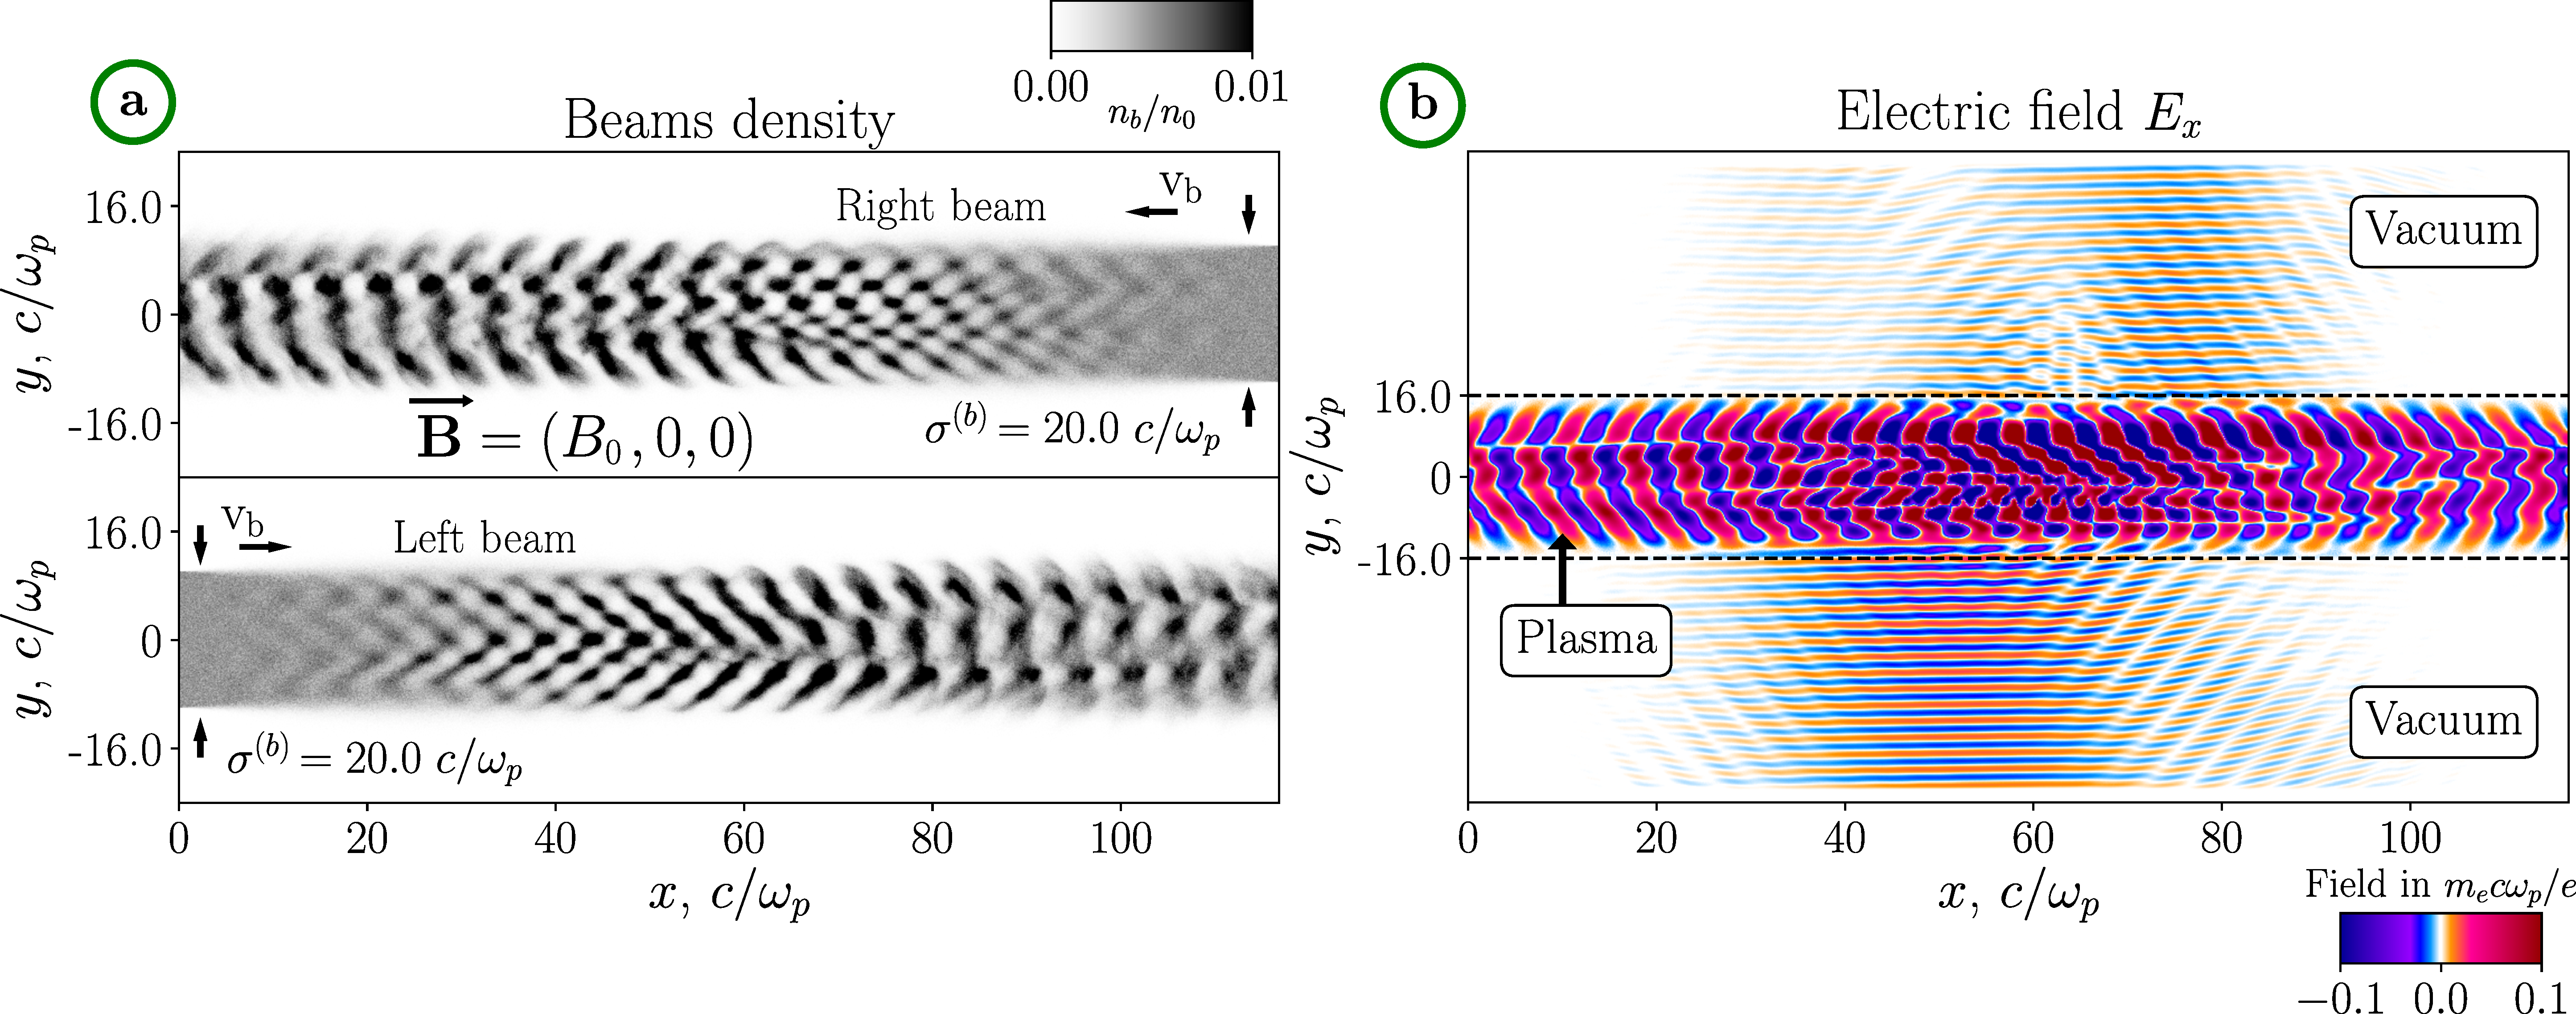
\includegraphics[width=0.45\linewidth]{fig2.pdf}
	\caption{Одна картинка по центру размером 0.45 длины строки}
	\label{fig:App1}%ссылка на картинку
\end{figure}

Ссылка на картинку в Приложении: Рисунок~\ref{fig:App1}


\end{document}